\usubsection{Estados}
Se definen 8 estados $X$, $Y$ y $Z$. $X$ representa a $S_1$, $Y$ a $S_0$ y
$\overline{Z}$ a LOAD:
\begin{enumerate}[label*=\textbf{\alph*)}]
  \item $X=0$, $Y=0$, $Z=0$: Carga tiempo mínimo de paso vehicular.
  \item $X=0$, $Y=0$, $Z=1$: Espera tiempo mínimo de paso vehicular y opción de solicitud de paso.
  \item $X=0$, $Y=1$, $Z=0$: Carga de tiempo de paso restringido(luz amarilla vehicular).
  \item $X=0$, $Y=1$, $Z=1$: Espera tiempo de paso restringido.
  \item $X=1$, $Y=0$, $Z=0$: Carga de tiempo de paso peatonal.
  \item $X=1$, $Y=0$, $Z=1$: Espera tiempo de paso peatonal.
  \item $X=1$, $Y=1$, $Z=0$: Carga de tiempo de banda de seguridad(luz roja vehicular y luz roja peatonal).
  \item $X=1$, $Y=1$, $Z=1$: Espera tiempo de banda de seguridad.
\end{enumerate}

\usubsection{Tabla de Estados}

\begin{table}[H]
  \centering
  \begin{tabular}{c c c c c}
    \toprule
    \multirow{2}{*}{EP}  & \multicolumn{4}{c}{Próximo Estado} \\
    & \multicolumn{4}{c}{Entradas: ZERO, SP'} \\  \cmidrule{2-5}
    XYZ & 00 & 01 & 10 & 11\\ \toprule
    a = 000 & 001 & 001 & 001 & 001\\ \midrule
    b = 001 & 001 & 001 & 001 & 010\\ \midrule
    c = 010 & 011 & 011 & 011 & 011\\ \midrule
    d = 011 & 011 & 011 & 100 & 100\\ \midrule
    e = 100 & 101 & 101 & 101 & 101\\ \midrule
    f = 101 & 101 & 101 & 111 & 110\\ \midrule
    g = 110 & 111 & 111 & 111 & 111\\ \midrule
    h = 111 & 111 & 111 & 000 & 000\\ \bottomrule
  \end{tabular}
\end{table}

\usubsection{Entradas}

\usubsubsection{Tabla de Excitación}

\begin{table}[H]
  \centering
  \begin{tabular}{c c c c c c c c c c c c}
    \toprule
    EP & X & Y & Z & ZERO & SP' & $J_X$ & $K_X$   & $J_Y$ & $K_Y$   & $J_Z$ & $K_Z$ \\
    \toprule
    a
       & 0 & 0 & 0 & x & x
       & 0 & x % JK X
       & 0 & x % JK Y
       & 1 & x % JK Z
       \\
    \cmidrule(r){1-6}      \cmidrule(l){7-8} \cmidrule(l){9-10} \cmidrule(l){11-12}
    \multirow{3}{*}{b}
       & 0 & 0 & 1 & 0 & x
       & \multirow{2}{*}{0} & \multirow{2}{*}{x} % JK X
       & \multirow{2}{*}{0} & \multirow{2}{*}{x} % JK Y
       & \multirow{2}{*}{x} & \multirow{2}{*}{0} % JK Z
       \\
       & 0 & 0 & 1 & 1 & 0 & & & & & &
       \\
    \cmidrule(r){2-6}      \cmidrule(l){7-8} \cmidrule(l){9-10} \cmidrule(l){11-12}
       & 0 & 0 & 1 & 1 & 1
       & 0 & x % JK X
       & 1 & x % JK Y
       & x & 1 % JK Z
       \\
    \cmidrule(r){1-6}      \cmidrule(l){7-8} \cmidrule(l){9-10} \cmidrule(l){11-12}
    c
       & 0 & 1 & 0 & x & x
       & 0 & x % JK X
       & x & 0 % JK Y
       & 1 & x % JK Z
       \\
    \cmidrule(r){1-6}      \cmidrule(l){7-8} \cmidrule(l){9-10} \cmidrule(l){11-12}
    \multirow{2}{*}{d}
       & 0 & 1 & 1 & 0 & x
       & 0 & x % JK X
       & x & 0 % JK Y
       & x & 0 % JK Z
       \\
    \cmidrule(r){2-6}      \cmidrule(l){7-8} \cmidrule(l){9-10} \cmidrule(l){11-12}
       & 0 & 1 & 1 & 1 & x
       & 1 & x % JK X
       & x & 1 % JK Y
       & x & 1 % JK Z
       \\
    \cmidrule(r){1-6}      \cmidrule(l){7-8} \cmidrule(l){9-10} \cmidrule(l){11-12}
    e
       & 1 & 0 & 0 & x & x
       & x & 0 % JK X
       & 0 & x % JK Y
       & 1 & x % JK Z
       \\
    \cmidrule(r){1-6}      \cmidrule(l){7-8} \cmidrule(l){9-10} \cmidrule(l){11-12}
    \multirow{2}{*}{f}
       & 1 & 0 & 1 & 0 & x
       & x & 0 % JK X
       & 0 & x % JK Y
       & x & 0 % JK Z
       \\
    \cmidrule(r){2-6}      \cmidrule(l){7-8} \cmidrule(l){9-10} \cmidrule(l){11-12}
       & 1 & 0 & 1 & 1 & x
       & x & 0 % JK X
       & 1 & x % JK Y
       & x & 1 % JK Z
       \\
    \cmidrule(r){1-6}      \cmidrule(l){7-8} \cmidrule(l){9-10} \cmidrule(l){11-12}
    g  & 1 & 1 & 0 & x & x
       & x & 0 % JK X
       & x & 0 % JK Y
       & 1 & x % JK Z
       \\
    \cmidrule(r){1-6}      \cmidrule(l){7-8} \cmidrule(l){9-10} \cmidrule(l){11-12}
    \multirow{2}{*}{h}
       & 1 & 1 & 1 & 0 & x
       & x & 0 % JK X
       & x & 0 % JK Y
       & x & 0 % JK Z
       \\
    \cmidrule(r){2-6}      \cmidrule(l){7-8} \cmidrule(l){9-10} \cmidrule(l){11-12}
       & 1 & 1 & 1 & 1 & x
       & x & 1 % JK X
       & x & 1 % JK Y
       & x & 1 % JK Z
       \\
    \bottomrule
  \end{tabular}
\end{table}

\usubsection{Solución mediante Mapas de Karnaugh}

% Copyright 2017 Emilio Rojas
%
% Permission is hereby granted, free of charge, to any person obtaining a copy of
% this software and associated documentation files (the "Software"), to deal in
% the Software without restriction, including without limitation the rights to
% use, copy, modify, merge, publish, distribute, sublicense, and/or sell copies of
% the Software, and to permit persons to whom the Software is furnished to do so,
% subject to the following conditions:
%
% The above copyright notice and this permission notice shall be included in all
% copies or substantial portions of the Software.
%
% THE SOFTWARE IS PROVIDED "AS IS", WITHOUT WARRANTY OF ANY KIND, EXPRESS OR
% IMPLIED, INCLUDING BUT NOT LIMITED TO THE WARRANTIES OF MERCHANTABILITY, FITNESS
% FOR A PARTICULAR PURPOSE AND NONINFRINGEMENT. IN NO EVENT SHALL THE AUTHORS OR
% COPYRIGHT HOLDERS BE LIABLE FOR ANY CLAIM, DAMAGES OR OTHER LIABILITY, WHETHER
% IN AN ACTION OF CONTRACT, TORT OR OTHERWISE, ARISING FROM, OUT OF OR IN
% CONNECTION WITH THE SOFTWARE OR THE USE OR OTHER DEALINGS IN THE SOFTWARE.

\textbf{Flip Flop $\text{J}_X$}
\begin{figure}[H]
  \centering
  \begin{subfigure}{0.1\textwidth}
    \centering
    \begin{tikzpicture}[scale=0.8]
      \draw(0,0) -- (0,0);
    \end{tikzpicture}
  \end{subfigure}
  \begin{subfigure}{.4\textwidth}
    \centering
    \begin{Karnaugh}{Y}{Z}{ZERO}{SP'}
      \minterms{14, 15}
      \implicant{15}{14}{blue}
    \end{Karnaugh}
  \end{subfigure}
  \begin{subfigure}{.4\textwidth}
    \centering
    \begin{Karnaugh}{Y}{Z}{ZERO}{SP'}
      \indeterminats{0, 1, 2, 3, 4, 5, 6, 7, 8, 9, 10, 11, 12, 13, 14, 15}
      \implicant{15}{14}{blue}
    \end{Karnaugh}
  \end{subfigure}

  \begin{subfigure}{0.5\textwidth}
    \centering
    \begin{tikzpicture}[scale=0.8]
      \draw(0,0) -- (0,0);
    \end{tikzpicture}
  \end{subfigure}
  \begin{subfigure}{.4\textwidth}
    \centering
    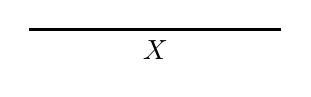
\begin{tikzpicture}[scale=0.8]
      \draw[very thick] (0,0.3) -- node [below]{$X$} ++(4,0);
    \end{tikzpicture}
  \end{subfigure}
  \caption*{$J_X = \color{blue} \text{Y} \cdot \text{Z} \cdot \text{ZERO}$.}
\end{figure}

\textbf{Flip Flop $\text{K}_X$}
\begin{figure}[H]
  \centering
  \begin{subfigure}{0.1\textwidth}
    \centering
    \begin{tikzpicture}[scale=0.8]
      \draw(0,0) -- (0,0);
    \end{tikzpicture}
  \end{subfigure}
  \begin{subfigure}{.4\textwidth}
    \centering
    \begin{Karnaugh}{Y}{Z}{ZERO}{SP'}
      \indeterminats{0, 1, 2, 3, 4, 5, 6, 7, 8, 9, 10, 11, 12, 13, 14, 15}
      \implicant{15}{14}{blue}
    \end{Karnaugh}
  \end{subfigure}
  \begin{subfigure}{.4\textwidth}
    \centering
    \begin{Karnaugh}{Y}{Z}{ZERO}{SP'}
      \minterms{14, 15}
      \implicant{15}{14}{blue}
    \end{Karnaugh}
  \end{subfigure}

  \begin{subfigure}{0.5\textwidth}
    \centering
    \begin{tikzpicture}[scale=0.8]
      \draw(0,0) -- (0,0);
    \end{tikzpicture}
  \end{subfigure}
  \begin{subfigure}{.4\textwidth}
    \centering
    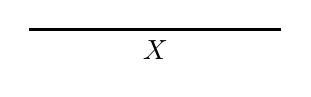
\begin{tikzpicture}[scale=0.8]
      \draw[very thick] (0,0.3) -- node [below]{$X$} ++(4,0);
    \end{tikzpicture}
  \end{subfigure}

  \caption*{$K_X = \color{blue} \text{Y} \cdot \text{Z} \cdot \text{ZERO}$.}
\end{figure}

\textbf{J}
\begin{figure}[H]
  \centering
  \begin{subfigure}{0.1\textwidth}
    \centering
    \begin{tikzpicture}[scale=0.8]
      \draw(0,0) -- (0,0);
    \end{tikzpicture}
  \end{subfigure}
  \begin{subfigure}{.4\textwidth}
    \centering
    \begin{Karnaugh}{Y}{Z}{ZERO}{SP'}
      \minterms{7}
      \indeterminats{8, 9, 10, 11, 12, 13, 14, 15}
      \implicant[3pt]{7}{15}{blue}
    \end{Karnaugh}
  \end{subfigure}
  \begin{subfigure}{.4\textwidth}
    \centering
    \begin{Karnaugh}{Y}{Z}{ZERO}{SP'}
      \minterms{6, 7}
      \indeterminats{8, 9, 10, 11, 12, 13, 14, 15}
      \implicant[3pt]{7}{15}{blue}
      \implicant{7}{14}{red}
    \end{Karnaugh}
  \end{subfigure}

  \begin{subfigure}{0.5\textwidth}
    \centering
    \begin{tikzpicture}[scale=0.8]
      \draw(0,0) -- (0,0);
    \end{tikzpicture}
  \end{subfigure}
  \begin{subfigure}{.4\textwidth}
    \centering
    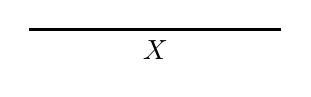
\begin{tikzpicture}[scale=0.8]
      \draw[very thick] (0,0.3) -- node [below]{$X$} ++(4,0);
    \end{tikzpicture}
  \end{subfigure}
  \caption*{$J_Y = \color{blue} \text{Z} \cdot \text{ZERO} \cdot \text{SP'} \color{black} + \color{red} \text{X} \cdot \text{Z} \cdot \text{ZERO} $.}
\end{figure}

\textbf{K}
\begin{figure}[H]
  \centering
  \begin{subfigure}{0.1\textwidth}
    \centering
    \begin{tikzpicture}[scale=0.8]
      \draw(0,0) -- (0,0);
    \end{tikzpicture}
  \end{subfigure}
  \begin{subfigure}{.4\textwidth}
    \centering
    \begin{Karnaugh}{Y}{Z}{ZERO}{SP'}
      \minterms{14, 15}
      \indeterminats{0, 1, 2, 3, 4, 5, 6, 7}
      \implicant{7}{14}{blue}
    \end{Karnaugh}
  \end{subfigure}
  \begin{subfigure}{.4\textwidth}
    \centering
    \begin{Karnaugh}{Y}{Z}{ZERO}{SP'}
      \minterms{14, 15}
      \indeterminats{0, 1, 2, 3, 4, 5, 6, 7}
      \implicant{7}{14}{blue}
    \end{Karnaugh}
  \end{subfigure}

  \begin{subfigure}{0.5\textwidth}
    \centering
    \begin{tikzpicture}[scale=0.8]
      \draw(0,0) -- (0,0);
    \end{tikzpicture}
  \end{subfigure}
  \begin{subfigure}{.4\textwidth}
    \centering
    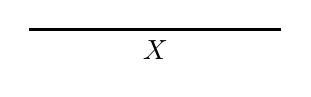
\begin{tikzpicture}[scale=0.8]
      \draw[very thick] (0,0.3) -- node [below]{$X$} ++(4,0);
    \end{tikzpicture}
  \end{subfigure}

  \caption*{$K_Y = \color{blue} \text{Z} \cdot \text{ZERO}$.}
\end{figure}

% Copyright 2017 Emilio Rojas
%
% Permission is hereby granted, free of charge, to any person obtaining a copy of
% this software and associated documentation files (the "Software"), to deal in
% the Software without restriction, including without limitation the rights to
% use, copy, modify, merge, publish, distribute, sublicense, and/or sell copies of
% the Software, and to permit persons to whom the Software is furnished to do so,
% subject to the following conditions:
%
% The above copyright notice and this permission notice shall be included in all
% copies or substantial portions of the Software.
%
% THE SOFTWARE IS PROVIDED "AS IS", WITHOUT WARRANTY OF ANY KIND, EXPRESS OR
% IMPLIED, INCLUDING BUT NOT LIMITED TO THE WARRANTIES OF MERCHANTABILITY, FITNESS
% FOR A PARTICULAR PURPOSE AND NONINFRINGEMENT. IN NO EVENT SHALL THE AUTHORS OR
% COPYRIGHT HOLDERS BE LIABLE FOR ANY CLAIM, DAMAGES OR OTHER LIABILITY, WHETHER
% IN AN ACTION OF CONTRACT, TORT OR OTHERWISE, ARISING FROM, OUT OF OR IN
% CONNECTION WITH THE SOFTWARE OR THE USE OR OTHER DEALINGS IN THE SOFTWARE.


\textbf{Flip Flop $\text{J}_Z$}
\begin{figure}[H]
  \centering
  \begin{subfigure}{0.1\textwidth}
    \centering
    \begin{tikzpicture}[scale=0.8]
      \draw(0,0) -- (0,0);
    \end{tikzpicture}
  \end{subfigure}
  \begin{subfigure}{.4\textwidth}
    \centering
    \begin{Karnaugh}{Y}{Z}{ZERO}{SP'}
      \minterms{0, 1, 2, 3, 8, 9, 10, 11}
      \indeterminats{4, 5, 6, 7, 12, 13, 14, 15}
      \implicant{0}{10}{blue}
    \end{Karnaugh}
  \end{subfigure}
  \begin{subfigure}{.4\textwidth}
    \centering
    \begin{Karnaugh}{Y}{Z}{ZERO}{SP'}
      \minterms{0, 1, 2, 3, 8, 9, 10, 11}
      \indeterminats{4, 5, 6, 7, 12, 13, 14, 15}
      \implicant{0}{10}{blue}
    \end{Karnaugh}
  \end{subfigure}

  \begin{subfigure}{0.5\textwidth}
    \centering
    \begin{tikzpicture}[scale=0.8]
      \draw(0,0) -- (0,0);
    \end{tikzpicture}
  \end{subfigure}
  \begin{subfigure}{.4\textwidth}
    \centering
    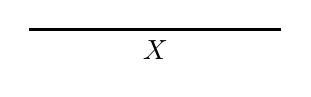
\begin{tikzpicture}[scale=0.8]
      \draw[very thick] (0,0.3) -- node [below]{$X$} ++(4,0);
    \end{tikzpicture}
  \end{subfigure}
  \caption*{$J_Z = 1$.}
\end{figure}

\textbf{Flip Flop $\text{K}_Z$}
\begin{figure}[H]
  \centering
  \begin{subfigure}{0.1\textwidth}
    \centering
    \begin{tikzpicture}[scale=0.8]
      \draw(0,0) -- (0,0);
    \end{tikzpicture}
  \end{subfigure}
  \begin{subfigure}{.4\textwidth}
    \centering
    \begin{Karnaugh}{Y}{Z}{ZERO}{SP'}
      \minterms{7, 14, 15}
      \indeterminats{0, 1, 2, 3, 8, 9, 10, 11}
      \implicantdaltbaix{0}{10}{blue}
      \implicant[3pt]{3}{11}{red}
      \implicant[6pt]{15}{10}{green}
    \end{Karnaugh}
  \end{subfigure}
  \begin{subfigure}{.4\textwidth}
    \centering
    \begin{Karnaugh}{Y}{Z}{ZERO}{SP'}
      \minterms{6, 7, 14, 15}
      \indeterminats{0, 1, 2, 3, 8, 9, 10, 11}
      \implicantdaltbaix{0}{10}{blue}
      \implicant[3pt]{3}{11}{red}
      \implicant[6pt]{15}{10}{green}
      \implicant[-2pt]{3}{10}{orange}
    \end{Karnaugh}
  \end{subfigure}

  \begin{subfigure}{0.5\textwidth}
    \centering
    \begin{tikzpicture}[scale=0.8]
      \draw(0,0) -- (0,0);
    \end{tikzpicture}
  \end{subfigure}
  \begin{subfigure}{.4\textwidth}
    \centering
    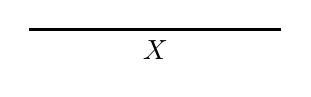
\begin{tikzpicture}[scale=0.8]
      \draw[very thick] (0,0.3) -- node [below]{$X$} ++(4,0);
    \end{tikzpicture}
  \end{subfigure}

  \caption*{$K_Z = \color{blue} \overline{\text{Z}} \color{black} + \color{red} \text{ZERO} \cdot \text{SP'} \color{black} + \color{green} \text{Y} \cdot \text{ZERO} \color{black} + \color{orange} \text{X} \cdot \text{ZERO}$.}
\end{figure}


\usubsection{Salidas}
  Ya se tienen las salidas $S_1$, $S_0$ y LOAD. Se puede deducir que SE solo se activa en \textbf{f}, por lo que su función
  es $X \overline{Y} Z$. Para TS tenemos la siguiente tabla de verdad y mapa de Karnaugh, de donde
  TS es $\text{Y}$
  \begin{figure}[H]
    \begin{subfigure}{0.49\textwidth}
      \centering
      \begin{tabular}{c c c | c}
        \toprule
        $X$ & $Y$ & $Z$ & TS \\ \midrule
        0     & 0     & 0   & 0 \\
        0     & 0     & 1   & x \\
        0     & 1     & 0   & 1 \\
        0     & 1     & 1   & x \\
        1     & 0     & 0   & 0 \\
        1     & 0     & 1   & x \\
        1     & 1     & 0   & 1 \\
        1     & 1     & 1   & x \\
        \bottomrule
      \end{tabular}
    \end{subfigure}
    \begin{subfigure}{0.49\textwidth}
      \centering
      \begin{Karnaughvuit}{X}{Y}{Z}
        \minterms{2, 6}
        \indeterminats{1, 3, 5, 7}
        \implicant{3}{6}{blue}
      \end{Karnaughvuit}
    \end{subfigure}
  \end{figure}


  \begin{figure}[H]
    \begin{subfigure}{0.49\textwidth}
      \centering
      \begin{tabular}{c c c | c}
        \toprule
        $X$ & $Y$ & $Z$ & LOAD \\ \midrule
        0     & 0     & 0   & 1 \\
        0     & 0     & 1   & 0 \\
        0     & 1     & 0   & 1 \\
        0     & 1     & 1   & x \\
        1     & 0     & 0   & 0 \\
        1     & 0     & 1   & x \\
        1     & 1     & 0   & 1 \\
        1     & 1     & 1   & x \\
        \bottomrule
      \end{tabular}
    \end{subfigure}
    \begin{subfigure}{0.49\textwidth}
      \centering
      \begin{Karnaughvuit}{X}{Y}{Z}
        \minterms{2, 6}
        \indeterminats{1, 3, 5, 7}
        \implicant{3}{6}{blue}
      \end{Karnaughvuit}
    \end{subfigure}
  \end{figure}
